\chapter{Hückel Theory and Conjugated Systems}\label{ch:b2:huckel}

Add hydrogen to cyclohexene and \qty{119}{kJ} are released per mole. Benzene,
with three double bonds in a ring of six carbons, should release three times
as much on its way to cyclohexane; it releases \qty{150}{kJ} less. That missing
energy is the stability of an \omterm{def:b2:huckel:aromatic}{aromatic} ring, the reason why benzene resists
the additions that alkenes undergo. In 1931 Erich Hückel computed it with a
determinant, after reducing the molecule to its $\pi$ electrons and their
neighbours. His method is crude, but it explains why rings of six $\pi$
electrons are special, why long conjugated chains absorb visible light, and
where a conjugated molecule carries its charges.

\begin{recall}
\Cref{ch:b2:diatomic-mos}: \omterm{def:b2:diatomic-mos:integrals}{Coulomb integral} $\alpha$, \omterm{def:b2:diatomic-mos:integrals}{resonance integral} $\beta$,
\omterm{def:b2:diatomic-mos:integrals}{secular determinant}. \Cref{ch:b2:fragment-orbitals}: $\pi$ orbitals of ethene and
allyl. The Year 1 volume: conjugated systems, resonance, chromophores and
absorption maxima.
\end{recall}

\section{The Hückel method}

In a planar conjugated molecule, the $\sigma$ orbitals are symmetric and the p
orbitals perpendicular to the plane antisymmetric with respect to that plane: they
do not mix (\cref{prop:b2:diatomic-mos:symmetry}), and the $\pi$ electrons can be
treated on their own.

\begin{definition}[Hückel method]\label{def:b2:huckel:method}
The \emph{Hückel method}\index{Hückel method} computes the $\pi$ orbitals of a
planar conjugated system as combinations $\psi = \sum_r c_r p_r$ of one p orbital per
atom, with the approximations: overlaps $S_{rs} = 0$ for $r \neq s$ (and 1 for $r =
s$); \omterm{def:b2:diatomic-mos:integrals}{Coulomb integrals} all equal to $\alpha$; \omterm{def:b2:diatomic-mos:integrals}{resonance integrals} equal to $\beta < 0$
between bonded neighbours and zero otherwise.
\end{definition}

With $x = (\alpha - E)/\beta$, the secular equations become, for each atom $r$,
$xc_r + \sum_{s \text{ bonded to } r} c_s = 0$, and the energies are the roots of a
determinant with $x$ on the diagonal and 1 between bonded atoms. Equivalently, $E =
\alpha + m\beta$ where the $m$ are the eigenvalues of the adjacency matrix of the
molecule's carbon skeleton; since $\beta < 0$, a positive $m$ is a bonding level.

\begin{method}[A Hückel calculation]\label{met:b2:huckel:huckel}
\begin{enumerate}
  \item Number the conjugated atoms; write the matrix with 0 on the diagonal and 1
        for each bonded pair.
  \item Find its eigenvalues $m_k$ (by the closed forms below, or numerically): $E_k =
        \alpha + m_k\beta$.
  \item Fill the levels from the most bonding, two electrons each:
        $E_\pi = \sum_k n_k E_k$.
  \item From the normalised coefficients, compute charges and bond indices.
\end{enumerate}
\end{method}

\begin{proposition}[Trace]\label{prop:b2:huckel:trace}
The energies of the $n$ $\pi$ orbitals of a Hückel system add up to $n\alpha$.
\end{proposition}

\begin{proof}
The sum of the eigenvalues of a matrix is its trace; the Hückel matrix has $\alpha$
on each of its $n$ diagonal entries.
\end{proof}

\section{Linear polyenes}

\begin{theorem}[Levels of a linear chain]\label{thm:b2:huckel:polyene}
A linear conjugated chain of $n$ atoms has the levels and coefficients
\[
  E_k = \alpha + 2\beta\cos\frac{k\pi}{n + 1}, \qquad
  c_{jk} = \sqrt{\frac{2}{n + 1}}\,\sin\frac{jk\pi}{n + 1}, \qquad k = 1, \dots, n .
\]
\end{theorem}

\begin{proof}
The secular equations are $c_{j-1} + xc_j + c_{j+1} = 0$ for $j = 1, \dots, n$, with
$c_0 = c_{n+1} = 0$. Try $c_j = \sin j\theta$: $\sin(j - 1)\theta + \sin(j + 1)\theta = 2\sin
j\theta\cos\theta$, so the equations hold with $x = -2\cos\theta$, and $c_0 = 0$
automatically. The end condition $c_{n+1} = \sin(n + 1)\theta = 0$ gives $\theta =
k\pi/(n + 1)$. Then $E = \alpha - x\beta = \alpha + 2\beta\cos\theta$. The normalisation uses
$\sum_{j=1}^n\sin^2 j\theta = (n + 1)/2$.
\end{proof}

\begin{example}[Butadiene]\label{ex:b2:huckel:butadiene}
For $n = 4$: $E = \alpha \pm 1.618\beta$, $\alpha \pm 0.618\beta$. Four $\pi$ electrons fill the two
bonding levels: $E_\pi = 4\alpha + 2(1.618 + 0.618)\beta = 4\alpha + 4.472\beta$. The lowest
orbital has coefficients 0.372, 0.602, 0.602, 0.372, the next 0.602, 0.372,
$-0.372$, $-0.602$.
\end{example}

\begin{omfigure}
\begin{tikzpicture}[font=\small]
  \foreach \k/\a/\b/\c/\d/\lab in {1/0.372/0.602/0.602/0.372/{$\psi_1$, $\alpha + 1.618\beta$},
      2/0.602/0.372/-0.372/-0.602/{$\psi_2$, $\alpha + 0.618\beta$},
      3/0.602/-0.372/-0.372/0.602/{$\psi_3$, $\alpha - 0.618\beta$},
      4/0.372/-0.602/0.602/-0.372/{$\psi_4$, $\alpha - 1.618\beta$}} {
    \begin{scope}[yshift={(\k-1)*2.1cm}]
      \draw[black!40] (-0.2,0) -- (3.2,0);
      \pic at (0,0) {omp={1.6*\a}{90}}; \pic at (1,0) {omp={1.6*\b}{90}};
      \pic at (2,0) {omp={1.6*\c}{90}}; \pic at (3,0) {omp={1.6*\d}{90}};
      \node[anchor=west] at (3.6,0) {\lab};
    \end{scope}
  }
\end{tikzpicture}

{\small The four $\pi$ orbitals of butadiene, lobes drawn in proportion to the
Hückel coefficients (computed) and coloured by their sign; energies increase
upwards, with $0, 1, 2, 3$ nodes. The two lower orbitals are filled.}
\end{omfigure}

\begin{definition}[$\pi$ charges and bond indices]\label{def:b2:huckel:indices}
With $n_k$ electrons in orbital $k$ (0, 1 or 2) and real coefficients $c_{rk}$, the
\emph{$\pi$ charge}\index{pi charge@$\pi$ charge} on atom $r$ is $q_r = \sum_k n_kc_{rk}^2$ (the
number of $\pi$ electrons it carries), and the \emph{$\pi$ bond index}\index{pi bond index@$\pi$ bond index}
of the bond $rs$ is $p_{rs} = \sum_k n_kc_{rk}c_{sk}$.
\end{definition}

For butadiene, $p_{12} = 2(0.372 \times 0.602 + 0.602 \times 0.372) = 0.894$ and $p_{23} =
2(0.602^2 - 0.372^2) = 0.447$: the end bonds carry most of the $\pi$ bonding and are
the shorter, the central bond has partial double-bond character. All the charges are
1.

\begin{proposition}[Alternant hydrocarbons]\label{prop:b2:huckel:alternant}
In a neutral hydrocarbon whose conjugated atoms can be coloured in two sets with
no two neighbours of the same set (no odd ring), every $\pi$ charge equals 1.
\end{proposition}

\admitted

The result (Coulson and Rushbrooke) is checked on butadiene above and on benzene by
symmetry; it is the reason why such hydrocarbons have no permanent dipole from their
$\pi$ electrons.

\begin{definition}[Delocalisation energy]\label{def:b2:huckel:delocalisation}
The \emph{delocalisation energy}\index{delocalisation energy} of a conjugated
system is the difference between its $\pi$ energy and that of the same number of
isolated double bonds, each with $E_\pi = 2\alpha + 2\beta$.
\end{definition}

For butadiene it is $4.472\beta - 4\beta = 0.472\beta$; for hexatriene, $0.988\beta$.

\section{Rings and aromaticity}

\begin{theorem}[Levels of a ring]\label{thm:b2:huckel:ring}
A planar ring of $n$ conjugated atoms has the levels $E_k = \alpha + 2\beta\cos(2\pi k/n)$,
$k = 0, 1, \dots, n - 1$: one lowest level $\alpha + 2\beta$, then pairs of degenerate
levels, and for even $n$ one highest level $\alpha - 2\beta$.
\end{theorem}

\begin{proof}
In a ring every atom has two neighbours, with indices taken modulo $n$:
$c_{j-1} + xc_j + c_{j+1} = 0$ for all $j$ and $c_{j+n} = c_j$. Try $c_j = \mathrm e^{\mathrm
i jq}$: the equation gives $x = -(\mathrm e^{-\mathrm iq} + \mathrm e^{\mathrm iq}) = -2\cos q$,
and periodicity requires $nq = 2\pi k$. The levels $k$ and $n - k$ have the same
energy; their sum and difference are real orbitals. Only $k = 0$ (and $k = n/2$ for
even $n$) is single.
\end{proof}

\begin{corollary}[Frost's circle]\label{cor:b2:huckel:frost}
The levels of a ring are read on a circle of radius $2|\beta|$ centred at $\alpha$, in
which a regular $n$-gon is inscribed with one vertex at the bottom: each vertex is
at the height of a level.
\end{corollary}

\begin{proof}
The vertex $k$ of the polygon is at angle $-\pi/2 + 2\pi k/n$, at height
$-2|\beta|\cos(2\pi k/n) = 2\beta\cos(2\pi k/n)$ relative to the centre.
\end{proof}

\begin{omfigure}
\begin{tikzpicture}[font=\scriptsize]
  \foreach \n/\x/\name/\el in {4/0/{\ce{C4H4}}/4, 5/3.4/{\ce{C5H5-}}/6, 6/6.8/{\ce{C6H6}}/6, 7/10.2/{\ce{C7H7+}}/6} {
    \begin{scope}[xshift=\x cm]
      \draw[black!35] (0,0) circle (1.2);
      \draw[black!60] \foreach \k in {0,...,\the\numexpr\n-1\relax} { ({-90+360*\k/\n}:1.2) -- ({-90+360*(\k+1)/\n}:1.2) };
      \foreach \k in {0,...,\the\numexpr\n-1\relax} {
        \draw[very thick] ({1.2*cos(-90+360*\k/\n)-0.22},{1.2*sin(-90+360*\k/\n)}) -- ({1.2*cos(-90+360*\k/\n)+0.22},{1.2*sin(-90+360*\k/\n)});
      }
      \draw[densely dotted] (-1.5,0) -- (1.5,0);
      \node[font=\small] at (0,-1.75) {\name};
    \end{scope}
  }
  \node[anchor=east] at (-1.5,0) {$\alpha$};
  % electrons: C4H4 (2 + 1 + 1), others filled lowest three
  \foreach \x in {0,3.4,6.8,10.2} {
    \draw[-{Stealth[length=1mm]}, thick] ({\x-0.05},-1.32) -- ({\x-0.05},-1.08);
    \draw[-{Stealth[length=1mm]}, thick] ({\x+0.05},-1.08) -- ({\x+0.05},-1.32);
  }
  % six-electron rings: the lowest degenerate pair is filled
  \foreach \n/\x in {5/3.4, 6/6.8, 7/10.2} {
    \foreach \k in {1, \the\numexpr\n-1\relax} {
      \pgfmathsetmacro\ex{\x + 1.2*cos(-90 + 360*\k/\n)}
      \pgfmathsetmacro\ey{1.2*sin(-90 + 360*\k/\n)}
      \draw[-{Stealth[length=1mm]}, thick] ({\ex-0.05},{\ey-0.12}) -- ({\ex-0.05},{\ey+0.12});
      \draw[-{Stealth[length=1mm]}, thick] ({\ex+0.05},{\ey+0.12}) -- ({\ex+0.05},{\ey-0.12});
    }
  }
  % C4H4: one electron in each of the two nonbonding levels
  \draw[-{Stealth[length=1mm]}, thick] (1.2,-0.12) -- (1.2,0.12);
  \draw[-{Stealth[length=1mm]}, thick] (-1.2,-0.12) -- (-1.2,0.12);
\end{tikzpicture}

{\small Frost's circles. The vertices of each polygon, inscribed with a vertex at the
bottom in a circle of radius $2|\beta|$, give the levels of the ring. With six $\pi$
electrons, \ce{C5H5-}, \ce{C6H6} and \ce{C7H7+} fill the lowest level and one degenerate
pair: closed shells. Cyclobutadiene's four electrons leave two electrons in a
degenerate nonbonding pair (drawn).}
\end{omfigure}

\begin{definition}[Aromaticity]\label{def:b2:huckel:aromatic}
A cyclic, planar, fully conjugated system is \emph{aromatic}\index{aromatic} when
its $\pi$ electrons form a closed shell with a large \omterm{def:b2:huckel:delocalisation}{delocalisation energy}, and
\emph{antiaromatic}\index{antiaromatic} when its $\pi$ electrons half-fill a degenerate
pair, which makes it less stable than the corresponding open chain.
\end{definition}

\begin{theorem}[Hückel's rule]\label{thm:b2:huckel:huckel-rule}
A planar monocyclic conjugated system has a closed shell of $\pi$ electrons if and only
if it holds $4N + 2$ of them ($N = 0, 1, 2, \dots$); with $4N$ it has two electrons in a
half-filled degenerate pair. This is \emph{Hückel's rule}\index{Hückel's rule}.
\end{theorem}

\begin{proof}
By \cref{thm:b2:huckel:ring}, the levels from the bottom are one single level and
then degenerate pairs (for the occupied part). A closed shell fills the single
level (2 electrons) and a whole number $N$ of pairs (4 electrons each): $4N + 2$. With
$4N$ electrons, the last pair holds only two, one in each of its orbitals (Hund's
rule).
\end{proof}

\begin{method}[Is it aromatic?]\label{met:b2:huckel:aromaticity}
\begin{enumerate}
  \item Is the system a ring with a p orbital on every atom (counting carbocation
        and carbanion centres and lone pairs of heteroatoms)?
  \item Can it be planar?
  \item Count the $\pi$ electrons: $4N + 2$ \omterm{def:b2:huckel:aromatic}{aromatic}, $4N$ \omterm{def:b2:huckel:aromatic}{antiaromatic} if planar.
  \item An \omterm{def:b2:huckel:aromatic}{antiaromatic} ring avoids planarity or conjugation when it can
        (cyclo-octatetraene is tub-shaped and behaves as a polyene).
\end{enumerate}
\end{method}

\begin{example}[Benzene]\label{ex:b2:huckel:benzene}
Six $\pi$ electrons fill $\alpha + 2\beta$ and the pair $\alpha + \beta$: $E_\pi = 6\alpha + 8\beta$.
Three isolated double bonds give $6\alpha + 6\beta$: the \omterm{def:b2:huckel:delocalisation}{delocalisation energy} is $2\beta$,
about twice that of the open chain of six carbons, hexatriene ($0.988\beta$): closing
the ring is worth as much again. By symmetry all bond indices are equal ($p = 2/3$), and so are the six
bond lengths, \qty{139.7}{pm}, between those of ethene (\qty{133.9}{pm}) and ethane
(\qty{153.6}{pm}).
% ledger: geo:C6H6.rCC, geo:C2H4.rCC, geo:C2H6.rCC
\end{example}

\begin{omfigure}
\begin{tikzpicture}[font=\small, y=0.013cm, x=1.0cm]
  \draw[thick] (0,0) -- (10.5,0);
  \node[anchor=north] at (5.2,-8) {cyclohexane ($\Delta_r H = 0$ reference)};
  % cyclohexene
  \draw[thick, omDef] (0.6,118.8) -- (1.6,118.8); \draw[->, omDef] (1.1,118.8) -- (1.1,4);
  \node[font=\scriptsize, anchor=south, align=center] at (1.1,120) {cyclohexene\\ \qty{118.8}{kJ/mol}};
  % diene
  \draw[thick, omDef] (3.6,227.7) -- (4.6,227.7); \draw[->, omDef] (4.1,227.7) -- (4.1,4);
  \draw[thick, black!45, densely dashed] (4.7,237.6) -- (5.6,237.6);
  \node[font=\scriptsize, anchor=south, black!60] at (5.15,240) {$2 \times 118.8$};
  \node[font=\scriptsize, anchor=east, align=right] at (3.5,227.7) {cyclohexa-1,3-diene\\ \qty{227.7}{kJ/mol}};
  % benzene
  \draw[thick, omDef] (7.6,206.0) -- (8.6,206.0); \draw[->, omDef] (8.1,206.0) -- (8.1,4);
  \node[font=\scriptsize, anchor=east, align=right] at (7.5,206.0) {benzene\\ \qty{206.0}{kJ/mol}};
  \draw[thick, black!45, densely dashed] (7.6,356.4) -- (8.6,356.4);
  \node[font=\scriptsize, anchor=south, black!60] at (8.1,358) {$3 \times 118.8 = 356.4$};
  \draw[<->, omThm, thick] (8.9,206) -- (8.9,356.4) node[midway, right, font=\scriptsize] {\qty{150}{kJ/mol}};
\end{tikzpicture}

{\small Enthalpies of hydrogenation to cyclohexane in the gas phase, from tabulated
enthalpies of formation (bars, height = heat released). Two conjugated double bonds
release \qty{10}{kJ/mol} less than twice one; benzene releases \qty{150}{kJ/mol} less than
three times one: its \omterm{def:b2:huckel:aromatic}{aromatic} stabilisation.}
% ledger: dfh:C6H6_g, dfh:C6H10_g, dfh:C6H12_g, dfh:C6H8_g
\end{omfigure}

\begin{history}[Kekulé's ring]
\begin{minipage}[t]{0.22\linewidth}
\vspace{0pt}
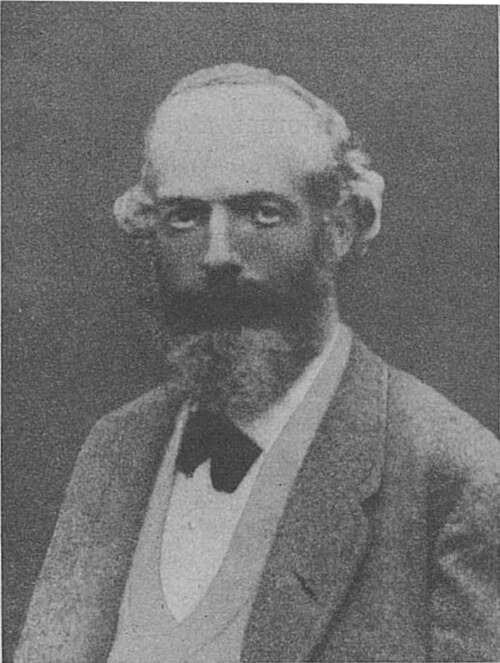
\includegraphics[width=\linewidth]{images/book3/kekule.jpg}
\end{minipage}\hfill
\begin{minipage}[t]{0.74\linewidth}
\vspace{0pt}
In 1865 August Kekulé proposed that the six carbon atoms of benzene form a ring
with alternating single and double bonds, and soon after that the two alternations
exchange so fast that every bond is the same. The equal bonds found by X-ray
diffraction, and the $\pi$ orbitals spread over the whole ring, gave his intuition its
modern form; \omterm{thm:b2:huckel:huckel-rule}{Hückel's rule}, in 1931, explained why six electrons, and not four or
eight, make a ring special. (Portrait, 1873, unknown author, public domain,
Wikimedia Commons.)
\end{minipage}
\end{history}

\section{Conjugation and light}

\begin{proposition}[The gap of a polyene]\label{prop:b2:huckel:gap}
In a linear polyene of $n$ carbons ($n$ even), the gap between the highest occupied
and the lowest empty $\pi$ level is $4|\beta|\sin(\pi/(2(n + 1)))$: it decreases as the
chain lengthens.
\end{proposition}

\begin{proof}
The highest occupied level is $k = n/2$, the lowest empty $k = n/2 + 1$. With $\theta_k =
k\pi/(n + 1)$, $E_{n/2+1} - E_{n/2} = 2|\beta|(\cos\theta_{n/2} - \cos\theta_{n/2+1}) = 4|\beta|
\sin\frac{\theta_{n/2} + \theta_{n/2+1}}{2}\sin\frac{\theta_{n/2+1} - \theta_{n/2}}{2}$, and the
first sine is $\sin(\pi/2) = 1$. It decreases with $n$ since $\sin$ increases on
$[0, \pi/2]$.
\end{proof}

\begin{omfigure}
\begin{tikzpicture}
\begin{axis}[width=0.5\linewidth, height=5cm, xmin=0, xmax=22, ymin=0, ymax=2.2,
  axis x line=bottom, axis y line=left, xlabel={carbons $n$}, ylabel={gap$/|\beta|$},
  tick label style={font=\small}, label style={font=\small}]
\addplot[omThm, thick, mark=*, mark size=1.3pt] table[x=n, y=gap] {figdata/out/bachelor-2-huckel-b.dat};
\end{axis}
\end{tikzpicture}\hfill
\begin{tikzpicture}
\begin{axis}[width=0.48\linewidth, height=5.4cm, xmin=-1, xmax=11, ymin=-2.4, ymax=2.4,
  axis x line=none, axis y line=left, ylabel={$(E - \alpha)/|\beta|$}, clip=false,
  tick label style={font=\small}, label style={font=\small}]
\addplot[only marks, mark=-, mark size=5pt, very thick, omDef] table[x=x, y=e] {figdata/out/bachelor-2-huckel-a.dat};
\draw[densely dotted] (axis cs:-1,0) -- (axis cs:11,0);
\node[anchor=north, font=\scriptsize] at (axis cs:0,-2.45) {C$_2$};
\node[anchor=north, font=\scriptsize] at (axis cs:2,-2.45) {C$_3$};
\node[anchor=north, font=\scriptsize] at (axis cs:4,-2.45) {C$_4$};
\node[anchor=north, font=\scriptsize] at (axis cs:6,-2.45) {C$_6$};
\node[anchor=north, font=\scriptsize] at (axis cs:8,-2.45) {ring 4};
\node[anchor=north, font=\scriptsize] at (axis cs:10,-2.45) {ring 6};
\end{axis}
\end{tikzpicture}

{\small Left: the Hückel gap of linear polyenes falls as the chain grows, the
reason why long conjugated chains absorb at longer wavelengths, up to the visible.
Right: computed levels of ethene, allyl, butadiene, hexatriene (chains) and of
cyclobutadiene and benzene (rings); bonding levels below $\alpha$.}
\end{omfigure}

A heteroatom is brought in by changing its \omterm{def:b2:diatomic-mos:integrals}{Coulomb integral}, $\alpha_X = \alpha + h\beta$, and the
\omterm{def:b2:diatomic-mos:integrals}{resonance integrals} of its bonds: a model with adjustable parameters, which keeps the
qualitative results (an electronegative atom, $h > 0$, draws the $\pi$ density towards
itself) but whose numbers are fitted, not derived.

\section{Exercises}

\begin{exercise}[$\star$]\label{exo:b2:huckel:1}
Give $E_\pi$ for the allyl cation, radical and anion.
\end{exercise}

\begin{exercise}[$\star$]\label{exo:b2:huckel:2}
Compute $E_\pi$ of butadiene from the levels $\alpha \pm 1.618\beta$, $\alpha \pm 0.618\beta$.
\end{exercise}

\begin{exercise}[$\star$]\label{exo:b2:huckel:3}
\omterm{def:b2:huckel:aromatic}{Aromatic}, \omterm{def:b2:huckel:aromatic}{antiaromatic} or neither (if planar): benzene, cyclopentadienyl anion,
cyclopentadienyl cation, tropylium cation \ce{C7H7+}, cyclobutadiene, planar
cyclo-octatetraene.
\end{exercise}

\begin{exercise}[$\star$]\label{exo:b2:huckel:4}
Draw Frost's circle for planar cyclo-octatetraene and place its eight $\pi$ electrons.
\end{exercise}

\begin{exercise}[$\star\star$]\label{exo:b2:huckel:5}
Compute the \omterm{def:b2:huckel:delocalisation}{delocalisation energy} of butadiene and give it in \unit{kJ/mol} with
$|\beta| = \qty{75}{kJ/mol}$. Compare with the \qty{10}{kJ/mol} of the hydrogenation
data for cyclohexa-1,3-diene.
\end{exercise}

\begin{exercise}[$\star\star$]\label{exo:b2:huckel:6}
Compute the $\pi$ bond indices of butadiene and predict which of its C--C bonds is the
shortest.
\end{exercise}

\begin{exercise}[$\star\star$]\label{exo:b2:huckel:7}
The levels of a five-membered ring are $\alpha + 2\beta$, $\alpha + 0.618\beta$ (twice),
$\alpha - 1.618\beta$ (twice). Fill them for the cyclopentadienyl anion and cation and
compare.
\end{exercise}

\begin{exercise}[$\star\star$]\label{exo:b2:huckel:8}
Using the levels of a seven-membered ring, explain why cycloheptatrienyl bromide
behaves as a salt, tropylium bromide.
\end{exercise}

\begin{exercise}[$\star\star$]\label{exo:b2:huckel:9}
Check the trace rule on hexatriene, whose levels are $\alpha \pm 1.802\beta$, $\alpha \pm
1.247\beta$, $\alpha \pm 0.445\beta$.
\end{exercise}

\begin{exercise}[$\star\star\star$]\label{exo:b2:huckel:10}
Derive the levels of hexatriene from the closed form, and its \omterm{def:b2:huckel:delocalisation}{delocalisation energy}.
\end{exercise}

\begin{exercise}[$\star\star\star$]\label{exo:b2:huckel:11}
Square cyclobutadiene would have two unpaired electrons. Explain why the real molecule
is rectangular, with two short and two long bonds.
\end{exercise}

\begin{exercise}[$\star\star\star$]\label{exo:b2:huckel:12}
In a two-atom $\pi$ system \ce{C=X} with $\alpha_X = \alpha + \beta$ (model value, $h = 1$) and
$\beta_{\ce{CX}} = \beta$, find the two levels and the $\pi$ charges on C and X for two
electrons.
\end{exercise}

\section{Problem: Benzene's Missing Energy}

\begin{problem}[{Weekend problem --- the aromatic stabilisation of benzene from
enthalpies of hydrogenation, the Hückel levels of benzene and its delocalisation
energy, the value of $|\beta|$, and the comparison with hexatriene and
cyclo-octatetraene}]
\label{pb:b2:huckel:1}
Data: enthalpies of formation of the gases (\unit{kJ/mol}): benzene 82.9,
cyclohexa-1,3-diene 104.6, cyclohexene $-4.3$, cyclohexane $-123.1$. Bond lengths
(pm): benzene 139.7, ethene 133.9, ethane 153.6.
% ledger: dfh:C6H6_g, dfh:C6H8_g, dfh:C6H10_g, dfh:C6H12_g, geo:C6H6.rCC, geo:C2H4.rCC, geo:C2H6.rCC

\medskip
\noindent\textbf{Part I --- Hydrogenation.}
\begin{enumerate}
  \item Compute $\Delta_r H^\circ$ of the hydrogenation of cyclohexene to cyclohexane.
  \item Same for cyclohexa-1,3-diene.
  \item Same for benzene.
  \item What would three independent double bonds release?
  \item Deduce the stabilisation of benzene.
  \item Compare with that of the conjugated diene, and comment.
\end{enumerate}

\medskip
\noindent\textbf{Part II --- Hückel benzene.}
\begin{enumerate}[resume]
  \item Write the Hückel matrix of benzene.
  \item Give its levels from the ring formula.
  \item Fill them with six $\pi$ electrons.
  \item Compute $E_\pi$.
  \item Compute $E_\pi$ of three isolated double bonds.
  \item Deduce the \omterm{def:b2:huckel:delocalisation}{delocalisation energy}.
  \item Check the trace rule.
\end{enumerate}

\medskip
\noindent\textbf{Part III --- The value of $|\beta|$.}
\begin{enumerate}[resume]
  \item Equate the \omterm{def:b2:huckel:delocalisation}{delocalisation energy} with the stabilisation of Part I and find
        $|\beta|$.
  \item With that value, predict the \omterm{def:b2:huckel:delocalisation}{delocalisation energy} of butadiene, and compare
        with Part I.
  \item Compute the $\pi$ bond indices of benzene.
  \item Compare them with those of butadiene.
  \item Explain why the bond lengths of benzene are equal and where they fall.
\end{enumerate}

\medskip
\noindent\textbf{Part IV --- Other rings and chains.}
\begin{enumerate}[resume]
  \item Compute the \omterm{def:b2:huckel:delocalisation}{delocalisation energy} of hexatriene and compare with benzene.
  \item Give the levels of planar cyclo-octatetraene.
  \item Fill them with eight electrons: what is wrong?
  \item How does the real molecule escape?
  \item What is the situation of cyclobutadiene?
  \item State \omterm{thm:b2:huckel:huckel-rule}{Hückel's rule}.
  \item State the value of $|\beta|$ obtained by matching benzene's \omterm{def:b2:huckel:delocalisation}{delocalisation energy}
        to its measured stabilisation.
\end{enumerate}
\end{problem}
